\chapter{Implementation}\label{ch:experiments}

This chapter describes how the design of \cref{ch:methods} was realised:
the representative system used for development, each implementation
stage with its code artefacts, and the concrete measurements obtained at
each stage.

\section{Representative System: CPSCore}\label{sec:cpscoreintro}

The pipeline was developed and validated on \emph{CPSCore}
\cite{theile:cpscore}, an open-source modular \Cpp\ framework for
cyber-physical systems originally built for the uavAP autopilot project.
It was chosen for three reasons: it is freely available, it uses a real
event-driven publish-subscribe architecture, and its test suite (1,425
assertions across 61 test cases) provides a ground truth for
behavioural verification.

\subsection{Scale and Dispatch Characteristics}\label{sec:cpscore-scale}

CPSCore is a small codebase: 154 source and header files, roughly
13,000 lines (3,800 in \texttt{.cpp} files, 9,200 in headers). It relies
heavily on \texttt{template}-based static polymorphism ($\approx$470
occurrences) and declares only 32 \texttt{virtual} method signatures
across 12 files, all confined to a single module (Utilities:
\texttt{INetworkLayer}, \texttt{ITransportLayer}, \texttt{IPublisherImpl},
\texttt{IScheduler}) or to per-module configuration boundaries
(\texttt{IConfigurableObject}, \texttt{IRunnableObject}). No
cross-module call resolves through a virtual table; inter-module calls
go through concrete class references or \texttt{boost::signals2} slot
connections.

This has a direct consequence for H1 (\cref{sec:h1-results}): since no
\emph{direct} cross-module call resolves through a virtual table, the
static call graph is reachability-complete with respect to the trace on
every genuine interaction reached through a direct call -- C2 has zero
recall gap on any true edge in S1, S2 and S4 (\cref{sec:h1-c4c2}). S3
is the one exception: one of its genuine edges is reached only through
a \texttt{std::function}-wrapped thread dispatch, a form of indirection
distinct from virtual dispatch that the static graph still cannot
resolve, giving C2 a real recall gap there (\cref{sec:h1-c4c2}). Neither
claim is a strict-subset claim ($\text{C3}\subseteq\text{C2}$), and
neither extends to false positives: on S1 and S4, C2 and C3 each carry
their own false-positive edge that the other source does not (C2's from
an unfiltered static over-approximation, C3's from an unfiltered
test-fixture-setup call in the trace), so C4's false-positive count is
strictly the sum of both, never a subset of either
(\cref{sec:h1-c4c2}). A codebase with pervasive cross-module virtual
dispatch or dynamic plugin loading would likely give static analysis a
recall gap on a wider range of scenarios than the single instance
(\texttt{std::function} dispatch) CPSCore exhibits here.

\subsection{CPSCore Architecture}

CPSCore is organised into five modules: \textbf{Aggregation} (component
wiring and lifecycle), \textbf{Configuration} (property mapping),
\textbf{Synchronization} (run-stage scheduling), \textbf{Logging}
(\texttt{CPSLogger}, \texttt{RAIILogStream}), and \textbf{Utilities}
(schedulers, data presentation, signal handling, \ac{IPC}, IDC).
External dependencies are Eigen3, Boost.System, \texttt{cpp\_redis}/tacopie,
and Catch2.

\subsection{Publish-Subscribe via IDC and Redis}\label{sec:idc}

Inter-component communication runs through the \ac{IDC} abstraction
layer, whose two operations (\texttt{subscribeOnPacket},
\texttt{sendPacket}) delegate to a pluggable \texttt{INetworkLayer}. The
default \texttt{RedisNetworkLayer} maps channel identifiers to
\texttt{RedisSubscriber}/\texttt{RedisPublisher} objects backed by
\texttt{cpp\_redis}, wired through a \texttt{boost::signals2} slot
(\texttt{onPacket\_.connect(slot)}) that fires when a Redis message
arrives -- the concrete instance of the call-site blind spot that
\cref{sec:macro-resolution} resolves.

\section{Phase 1 --- Static Analysis}\label{sec:static-impl}

\subsection{Renaissance to Neo4j}

CPSCore's source tree was analysed by Renaissance, which resolves the
full \ac{AST} (template instantiations, overload candidates, macro
expansions) and emits the property graph schema in
\cref{tab:node-types,tab:edge-types}: 11 node labels and 11 relationship
types, all from static analysis, populating a graph of 67,104 nodes.
Runtime traces are processed separately into a sequence table and
combined with the static edge set only at evaluation time
(\cref{sec:combine-scope}).

\subsection{Schema Introspection Skill}

The \texttt{get-neo4j-schema} skill runs three Cypher statements against
the live graph to produce a machine-readable schema summary for
downstream skills:

\begin{minted}{cypher}
-- Node labels and properties
CALL db.schema.nodeTypeProperties()
YIELD nodeType, propertyName, propertyTypes
RETURN nodeType, propertyName, propertyTypes;

-- Relationship types and properties
CALL db.schema.relTypeProperties()
YIELD relType, propertyName, propertyTypes
RETURN relType, propertyName, propertyTypes;

-- Relationship signatures (which label pairs each edge connects)
MATCH (s)-[r]->(t)
RETURN DISTINCT labels(s) AS fromLabels,
                type(r)   AS relType,
                labels(t) AS toLabels;
\end{minted}

\subsection{Scenario-Scoped Query}\label{sec:scenario-query-impl}

For a given scenario, \texttt{text-to-cypher} translates the scenario
description into a schema-aware Cypher query and \texttt{cypher-to-output}
executes it against the live graph, returning the scenario-scoped
subgraph consumed by Phase~1. For S1a/S1b, which share a component scope
(``Using agent skills, show me Synchronization calling into Aggregation
and Logging''):

\begin{minted}{cypher}
// scoped to S1a/S1b: Synchronization / Aggregation / Logging
MATCH (caller)-[:CppCalls]->(callee)
WHERE (caller.name CONTAINS '/src/Synchronization/'
    OR caller.name CONTAINS '/include/cpsCore/Synchronization/')
  AND (callee.name CONTAINS '/Aggregation/' OR callee.name CONTAINS '/Logging/')
RETURN DISTINCT
    caller.name AS callerName, caller.symbol AS callerSymbol,
    callee.name AS calleeName, callee.symbol AS calleeSymbol
\end{minted}

Before this query runs, the running example edge
\texttt{SynchronizedRunner.runSynchronized}~$\to$~\texttt{Aggregator.getAll}
exists in the graph only as a raw \texttt{CppCalls} relationship among
67,104 undifferentiated nodes, with a near-identical sibling edge to
\texttt{CPSLogger.flush} fired from the same call site; this query is
what carves the S1a/S1b-scoped subgraph out of the rest of the graph.

\subsection{Dependency Table Extraction}\label{sec:idt}

The \texttt{get-interface-dependency-table} skill queries Neo4j for all
11 relationship types and their permitted node-label pairs, producing a
compact schema summary used to ground the \texttt{text-to-cypher} skill
so that generated Cypher queries reference only valid edge types. The
resulting architectural dependency diagram was also presented to the
expert panel in the H3 evaluation (\cref{sec:h3}).

\section{Phase 2 --- Guided Instrumentation}\label{sec:trace-impl}

\subsection{Probe Insertion via csp\_matcher}\label{sec:trace-probe-insertion}

The \texttt{add-runtime-instrumentation} skill drives \texttt{csp\_matcher}
(\cref{sec:csp-matcher}) to wrap the cross-component call sites
identified above with a comma-operator trace emission, using the
find/replace rules in \texttt{add\_tracing.txt}: three call-site
patterns (\texttt{getAll}, \texttt{flush}, \texttt{convert}), one per
distinct cross-component call type the Cypher query surfaced, plus the
CPSLOG macro patch covering every \texttt{RAIILogStream::stream} call
site. \texttt{apply\_tracing.ps1} applies these across all compilation
units in \texttt{compile\_commands.json}:

\begin{minted}{cpp}
// Example wrapped call site in AggregatableRunner.cpp
(cspTrace("Synchronization", "Aggregation", "Aggregator.getAll"),
 agg->getAll<IAggregatableObject>())
\end{minted}

Each probe emits a structured, pipe-delimited \texttt{[TRACE]} line to
\texttt{stderr} when the call fires, capturing wall-clock timestamp,
caller/callee component, and function names (full rules in
\cref{sec:appendix-tracing-rules}). Because probes wrap call sites
rather than function entries, the trace records that a specific
cross-component call executed, not merely that a function was entered.

\subsection{Trace Format and Output}

\begin{minted}{text}
EventTimestamp | EventName | ClientComponent | ClientFunction
               | ServerComponent | ServerFunction
               | RelationshipType | InterfaceNames
\end{minted}

Running the CPSCore test suite under \texttt{csp\_matcher} instrumentation
produced 27 real trace events covering 26 unique client-to-server
interaction pairs, genuine runtime captures, not a static projection.
Example events:

\begin{minted}{text}
2026-06-18T10:07:15.686645Z | Aggregator.getAll |
  Synchronization | AggregatableRunner.notifyAggregationOnUpdate |
  Aggregation | Aggregator.getAll | Command | Aggregator

2026-06-18T10:07:15.694645Z | CPSLogger.flush |
  Synchronization | SynchronizedRunner.runSynchronized |
  Logging | CPSLogger.flush | Command | CPSLogger
\end{minted}

The full test run passed all 1,425 assertions (\cref{sec:cpscoreintro}),
confirming instrumentation did not alter runtime behaviour.

\section{Phase 3 --- Neo4j-Based Reachability Filter}\label{sec:synthesis-impl}

Phase~3 applies the Neo4j-based reachability filter
(\cref{sec:evidence-synthesis}) to each condition's trace input:
C5 filters \texttt{trace\_slice.txt}, C6 filters
\texttt{full\_trace.txt}, C4 reads \texttt{trace\_slice.txt} without
the filter, and C7--C9 pass C2, C3, and C4 candidate lists to a
two-prompt \ac{LLM} chain.

For CPSCore, \texttt{trace\_slice.txt} contains 8 sequence events and
both ground-truth interaction edges for S1a, and 5 sequence events and
3 interaction edges for S1b. Setup-phase events
(\texttt{Aggregator.add} firing before either runner starts) are
present in both traces and are removed by the C5 filter; S2 and S3
contain no setup-phase noise.

\section{Phase 4 --- SysML v2 Generation}\label{sec:sysml-impl}

For S1a, S1b, S2 and S3, the \texttt{draw-sysml-sequence-model} and
\texttt{draw-sysml-structural-model} skills read the \texttt{sequence.json}
and \texttt{interactions.json} files written by condition~C5
(guided+reachability)
and render each scenario as a \sysml \texttt{interaction} definition,
following the schemas in \cref{sec:sysml-generation}. The broader,
whole-codebase set of 14 auto-generated scenarios described below is a
separate, bulk visualisation: it is generated directly from the unscoped
Phase~1 CSV tables, bypassing scenario scoping and synthesis entirely,
and serves to illustrate coverage across CPSCore rather than to feed the
H1/H2 evaluation. The generated package declares shared stereotypes
(\texttt{SynchronousCall}, \texttt{ReturnMessage},
\texttt{AsynchronousMessage}) and one \texttt{part def} per scenario. An
excerpt from the generated \texttt{TestExecution} scenario:

\begin{minted}[fontsize=\footnotesize]{text}
package CPScoreInteractionModels {
    private import ScalarValues::String;

    part def SynchronousCall :> Message { ... }

    part def TestExecutionScenario :> InteractionScenario {

        part filterTest : Lifeline;
        part catch2     : Lifeline;
        part logger     : Lifeline;
        part enumMap    : Lifeline;

        part m1 : SynchronousCall {
            ref from : Lifeline = filterTest;
            ref to   : Lifeline = catch2;
            attribute :>> label = "1. complete";
        }
        part m6 : SynchronousCall {
            ref from : Lifeline = loggerTest;
            ref to   : Lifeline = logger;
            attribute :>> label = "6. instance";
        }
        ...
    }
}
\end{minted}

A separate \texttt{RedisConnectionScenario} covers the Redis
subscriber/publisher initialisation interactions
(\texttt{connect}, \texttt{auth}, \texttt{subscribe},
\texttt{onConnectionEvent}), spanning the \texttt{RedisPublisher},
\texttt{RedisSubscriber}, \texttt{CppRedisClient}, and \texttt{Logger}
lifelines.

\begin{figure}[htb]
\centering
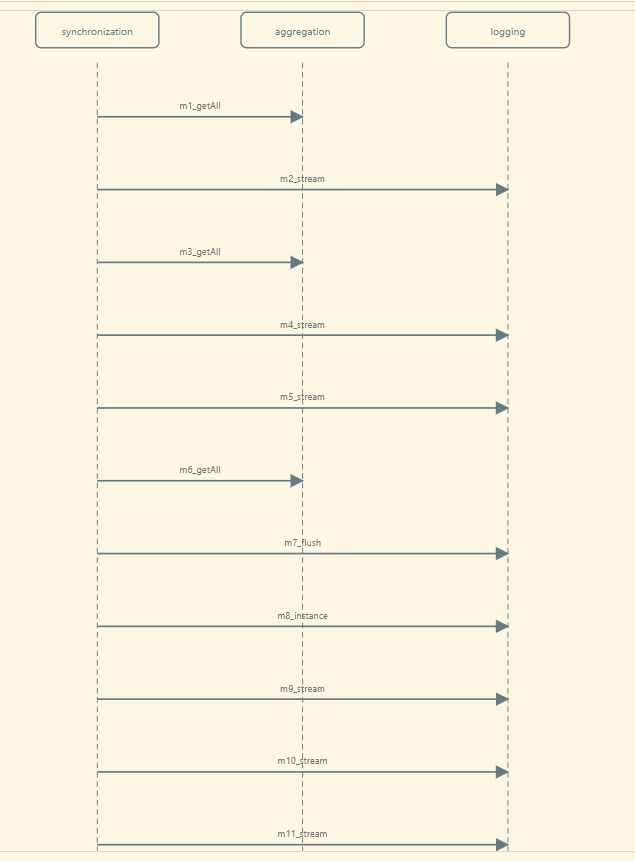
\includegraphics[width=0.85\textwidth]{figures/s1-sequence.png}
\caption{An example of the pipeline's final rendered output: the generated
  \sysml sequence diagram for the whole-codebase \emph{Aggregation}
  scenario, one of the 14 bulk-generated, unscoped diagrams described
  above. It is illustrative of output style and coverage only, not one
  of the scenario-scoped, per-condition reconstructions scored in
  \cref{sec:h1} (those are reproduced separately in
  \cref{sec:appendix-generated}). The complete set of bulk-generated
  diagrams is reproduced in \cref{sec:appendix-sysmlv2}.}
\label{fig:s1-sequence-main}
\end{figure}

The complete set of generated SysML v2 sequence and structural diagrams
is reproduced in \cref{sec:appendix-sysmlv2}, covering all 14
auto-generated scenarios (Aggregation, Synchronization, IDC, IPC, Redis,
Serial, Signal Handler, Utilities, Data Presentation, and Test Execution
flows).

\section{Scenario Suite and Experimental Conditions}\label{sec:scenario-suite}

The stages above produce the raw artefacts (the static sequence
dependency table and the real \texttt{csp\_matcher} trace log) feeding
the H1 and H2 experiments in \cref{ch:analysis}. This section documents
how those artefacts were assembled into experimental configurations.

\subsection{Scenario Suite (S1a, S1b, S2, S3)}\label{sec:scenarios}

Four scenarios were defined on CPSCore, all found-in-the-wild: each
corresponds to an existing Catch2 test case exercising a real
cross-component interaction, none constructed for this evaluation. Two
of them, S1a and S1b, exercise the same underlying call chain under
different test cases --- the happy path and the timeout branch of
\texttt{SynchronizedRunnerTest}, respectively --- covering both an
over-approximation blind spot in static analysis (S1a: C2 reports
extran\-eous static edges the trace never fires) and a runtime-suppression
blind spot in dynamic analysis (S1b: logging is suppressed by
\texttt{setLogLevel(NONE)}, so the timeout-warning interaction is visible
only to static analysis).

\begin{description}
  \item[S1a: Aggregator notification chain, happy path.]
    \emph{Primary:} Synchronization. \emph{Targets:} Aggregation, Logging.
    The observer/notification pattern exercised by
    \texttt{SynchronizedRunnerTest}: \texttt{SynchronizedRunner.runSynchronized}
    ~$\to$~\texttt{Aggregator.getAll}, followed by a logging call. The
    \texttt{boost::signals2} callback chain is invisible in a static
    include graph, making this a test of IDC topology recovery.
    \emph{Reference interactions:} 2 (getAll, flush).

  \item[S2: Configuration property mapping.]
    \emph{Primary:} Configuration. \emph{Target:} Logging. A mostly-static,
    linear chain: \texttt{PropertyMapper.add}~$\to$~\texttt{RAIILogStream.stream}.
    The easy-case baseline, expected to be reconstructed well even by
    static-only conditions. \emph{Reference interactions:} 1 (stream).

  \item[S3: Multi-component runner orchestration.]
    \emph{Primary:} Synchronization. \emph{Targets:} Aggregation, Utilities,
    Logging. Fan-out from \texttt{AggregatableRunner.runAllStages} /
    \texttt{notifyAggregationOnUpdate} to multiple independent
    subsystems at once, driven through
    \texttt{MultiThreadingScheduler.schedule/run/runSchedule/stop} and
    \texttt{ObjectHandleContainer.setFromAggregationIfNotSet}. The
    hardest case for static analysis: one of the three genuine
    cross-component calls (\texttt{Utilities}~$\to$~\texttt{Logging:stream})
    is dispatched through a \texttt{std::function}-wrapped thread with
    no resolvable static call site, so C2 misses it entirely -- a
    recall gap, not a false positive (C2's precision on S3 is 1.000; it
    reports zero extraneous edges, only an incomplete set). Intersection
    (C5) is therefore bounded by C2's recall on this scenario alone
    (\cref{sec:h1-c4c2}). \emph{Reference interactions:} 3
    (\texttt{Aggregation}~$\to$~\texttt{Logging:stream},
    \texttt{Synchronization}~$\to$~\texttt{Aggregation:getAll},
    \texttt{Utilities}~$\to$~\texttt{Logging:stream}); full listing in
    \cref{sec:appendix-groundtruth}.

  \item[S1b: Aggregator notification chain, timeout path.]
    \emph{Primary:} Synchronization. \emph{Targets:} Aggregation, Logging.
    The same call chain as S1a, exercised instead by the timeout branch
    of \texttt{SynchronizedRunnerTest}. The test suppresses all logging
    via \texttt{CPSLogger::instance()->setLogLevel(LogLevel::NONE)} before
    triggering the timeout, so the timeout-warning interaction
    (\texttt{SynchronizedRunnerMaster.runStage}~$\to$~\texttt{RAIILogStream.stream})
    is visible in C2's static call graph but absent from the unfiltered
    runtime trace (C3) --- a deliberate dynamic blind spot mirroring S1a's
    static over-approximation blind spot.
    \emph{Reference interactions:} 3 (getAll, flush, stream). As with
    S1a, \texttt{CPSLogger::instance()} is excluded from ground truth as
    a singleton accessor call rather than a genuine interaction
    (\cref{sec:idt}), and the \texttt{Aggregator.add}$\to$
    \texttt{RAIILogStream.stream} call that fires during test-fixture
    setup, before either runner starts, is excluded as out of the
    scenario's logical scope (\cref{sec:appendix-groundtruth}).
\end{description}

Each scenario's ground truth was first drawn by hand from direct source
inspection: the relevant directories, classes and call sites, together
with the test case that exercises them, and only then transcribed into
the \sysml textual reference diagrams used for scoring, keeping the
reference independent of the pipeline's own output. Both forms, for
all four scenarios, are reproduced in
\cref{sec:appendix-groundtruth}.

\subsection{Nine-Condition Design (C1--C9)}\label{sec:conditions}

Each scenario was reconstructed independently under nine conditions:

\begin{description}
  \item[C1: LLM-only.] Reconstruction by an \ac{LLM} reasoning over raw
    source code alone, with no access to the static graph or any trace,
    a baseline for what an agent can infer without the pipeline. As an
    Azure-OpenAI-backed condition it is not deterministically reproducible
    run-to-run, unlike C2--C6.
  \item[C2: Static-only.] Forward \texttt{CppCalls*0..8} traversal from
    scenario entry points in the Neo4j call graph, collecting
    cross-component edges in traversal order.
  \item[C3: Unfiltered dynamic trace.] All events from
    \texttt{full\_trace.txt} with no component-scope or reachability
    filter applied. Retains intra-component calls and setup-phase events,
    making this the noisiest dynamic baseline.
  \item[C4: Guided-only.] Events from \texttt{trace\_slice.txt}
    (instrumentation probes placed at Neo4j-identified architectural call
    sites only) with no further reachability filter. Setup-phase events
    can still fire at instrumented sites, so C4 retains some
    setup-phase false positives; it is otherwise clean.
  \item[C5: Guided~+~reachability.] \texttt{trace\_slice.txt} filtered
    by a Neo4j \texttt{CppCalls*0..8} reachability query scoped to
    \texttt{SCENARIO\_ENTRY} functions. Eliminates setup-phase false
    positives by keeping only events whose caller is reachable from the
    scenario entry point. Fully deterministic and reproducible.
  \item[C6: Full trace~+~reachability.] \texttt{full\_trace.txt} with the
    same reachability filter as C5. Ablation of C5 that tests whether
    the filter alone is sufficient regardless of instrumentation strategy.
  \item[C7: LLM~+~C2 candidates.] Two-prompt \ac{LLM} chain seeded with
    C2's static candidates: the first prompt filters static
    over-approxi\-mations and adds dynamically-dispatched calls; the
    second orders the sequence. Requires C2 output and Azure credentials.
  \item[C8: LLM~+~C3 candidates.] Same chain seeded with C3's
    unfiltered trace: the first prompt removes intra-component and
    setup-phase events and adds missed calls.
  \item[C9: LLM~+~C4 candidates.] Same chain seeded with C4's
    guided-trace candidates: the first prompt removes any residual
    setup-phase false positives and adds missed calls.
\end{description}

C1--C9 test \hyperref[sec:h1]{H1} (which evidence source, or combination
of sources, most accurately recovers interaction sets and execution
sequences). C4 and C5 isolate the contribution of the reachability
filter (C5 vs.~C4); C5 and C6 isolate the contribution of guided
instrumentation (C5 vs.~C6). C7, C8, and C9 assess whether \ac{LLM}
post-processing adds value when a prior is already available.
\hyperref[sec:h2]{H2} is tested separately, by the
guided-versus-full instrumentation comparison below
(\cref{sec:guided-vs-full}), not by any pair of the nine conditions
above.

\subsection{Guided versus Full Instrumentation}\label{sec:guided-vs-full}

H2 requires a second axis, orthogonal to the nine conditions above: how
the trace itself is collected.

\begin{description}
  \item[Full instrumentation.] \texttt{csp\_matcher} probes are inserted
    at every candidate call site in the static graph, independent of
    scenario.
  \item[Code-graph-guided instrumentation.] Probes are inserted only at
    call sites within the scenario scope (\cref{sec:scenario-scoping}),
    computed \emph{before} instrumentation rather than filtered after.
\end{description}

This is what makes the H2 comparison meaningful: whether using the code
graph to decide where to look produces a cleaner trace than
instrumenting everything and filtering afterwards, at equivalent or
better coverage. Results (node/edge/noise reduction, coverage) are
reported in \cref{sec:h2-results}.

\begin{table}[htb]
\centering
\caption{Quantitative outcomes per pipeline stage on CPSCore.}
\label{tab:impl-summary}
\begin{tabular}{@{} l r @{}}
\toprule
\textbf{Artefact} & \textbf{Count} \\
\midrule
Graph node labels                            & 11 \\
Graph relationship types                     & 11 \\
Sequence dependency table rows               & 2,574 \\
Unique client$\to$server function pairs (static) & 2,169 \\
Distinct components in sequence table        & 121 \\
Instrumentation targets (functions)          & 9 \\
Source files instrumented                    & 5 \\
Total trace events (csp\_matcher)             & 27 \\
Unique client$\to$server pairs (trace)        & 26 \\
SysML v2 scenarios generated                 & 14 \\
Test assertions passing post-instrumentation & 1,425 / 1,425 \\
\bottomrule
\end{tabular}
\end{table}
